\chapter{oMdu saraLa samaseyx}

\begin{center}
datatx Akaqtiyalilx eSuTx cwka matutx eSuTx AyatagaLirutatxve?
\end{center}

shirxV kaqSaNxsAvxmi utatxma shikaSxkaru. vidAyxthiRgaLige pirxyaru. oMdoMdu dinavU avara pAThaveMdare vidAyxthiRgaLige kutUhalaveV. aMdu shirxV subabxrAvf rajadalilxdadxru. avara taragatiyanunx shirxV kaqSaNxsAvxmi avarige muKayx shikaSxkaru vahisidadxru. kaqSaNxsAvxmi avaru taragatige hoVda meVle sumamxne kuLitukoLuLxva savxBAvadavaralalx. kapupxhalageya meVle oMdu cwkavanunx  baredu
\begin{tabular}{c}
\centering{\includegraphics{src/figures/square.eps}}
\end{tabular}
 ililx eSuTx cwkagaLive? eMdu parxshinxsidaru. vidAyxthiRgaLige AshacxyaR! cwkaviruvudu oMdeV, AdarU eSuTx cwkagaLive eMdaralAlx eMdu kumArf yoVcisi, iruvudeV oMdu cwkavalalxveV? eMda. sari kaqSaNxsAvxmi avaru
\begin{tabular}{c}
\centering{
\includegraphics{src/figures/rectangle.eps}}
\end{tabular} 
I Akaqtiyalilx eSuTx Ayatavide? eMdu\ parxshinxsidaru. vidAyxthiRgaLige punaH AshacxyaR ideVnidu? cwka baredu Ayata eSiTxde? eMdu keVLutitxdAdxralalx aMta. muMde kuLitidadx pAshA bahaLa budidhxvaMta. sArf oMdu Ayata ide eMda. guDf eMdaru. uLidavarige kutUhala. adu heVge? eMdaru. Aga kaqSaNxsAvxmigaLu cwkavU AyataveV. aBimuKa bAhugaLu parasapxra sama matutx samAnAMtaravAgiruva catuBuRja AyataveV eMdaru. sari muMduvariyutatx kaqSaNxsAvxmigaLu 
\begin{tabular}{ |l|l| }
  \hline
 {\;}  & {\;} \\ \hline
  & \\
  \hline
\end{tabular}
I riVtiya matotxMdu Akaqti baredu, idaralilx eSuTx cwkagaLive eMdaru. nAlukx eMdavareV hecucx jana Adare, sureVsha aidu cwkagaLive eMda. kapupxhalageya hatitxra avananunx karedu heVge toVriseMdaru? oMdu doDaDx, nAlukx cikakx cwkagaLanunx toVrisida. A doDaDx cwkavanunx seVrisabeVkeMdu yArigU hoLedititxlalx. AyatagaLeSiTxve? eMdAga taragatiyalilx nishashxbadx eNisalu AraMBisidaru. jAnf edudx niMtu {\rm 9} eMda kaqSaNxsAvxmigaLige saMtoVSavAyitu. I riVti AkaqtigaLalilx cwkagaLeSiTxve? AyatagaLeSiTxve? eMdu tiLisalu yAvudAdarU sUtarxvideyeV eMda rAmeVgwDa. kaqSaNxsAvxmigaLige vidAyxthiRgaLa samayoVcita parxshenx matatxSuTx saMtoVSa niVDitu.

$n^2$ cwkagaLanunx hoMdiruva oMdu Akaqtiyalilx $\dfrac{(n^2+n)^2}{4}$ Ayata\-gaLirutatxve.
avugaLalilx $\dfrac{2n^3+3n^2+n}{6}$ cwkagaLirutatxve. hAgU $\dfrac{3n^4+2n^3-3n^2-2n}{12}$
cwkagaLalalxda AyatagaLu irutatxve eMdaru. 

Iga niVvu koTiTxruva Akaqtige I sUtarxvanunx anavxyisidare eSuTx cwka, eSuTx Ayata barutatxde? eMda parameVsha. OhoV heVLitxVni noVDi

I Akaqtiyalilx $n=2$
$$
\text{AyatagaLu} =\dfrac{(n^2+n)^2}{4}=\dfrac{(2^2+2)^2}{4}=\dfrac{(4+2)^2}{4}=\dfrac{(6^2)}{4}=\dfrac{36}{4}=9
$$

I oTuTx {\rm 9} AyatagaLalilx kelavu cwkagaLu matetx kelavu cwkavalalxda Ayata
\begin{align*}
\text{cwkagaLu} \quad &\dfrac{2n^3+3n^2+n}{6}=\dfrac{2(2)^3+3(2)^2+n}{6} \hspace{2cm}\\
& =\dfrac{16+12+2}{6}=\dfrac{30}{6}=5
\end{align*}
\begin{align*}
\text{cwkagaLalalxda AyatagaLu}
 \quad &\dfrac{3n^4+2n^3-3n^2-2n}{12} \hspace{2cm}\\
&=\dfrac{3(2)^4+2(2)^3-3(2)^2-2(2)}{12}\\ 
 &=\dfrac{48+16-12-4}{12}=\dfrac{48}{12}=4
\end{align*}

oMdu shAleyalilx gaNitakekx saMbaMdhisidaMte oMdu rasa parxshenx mADide.
\begin{tabular}{c}
\centering{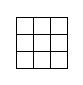
\includegraphics{src/figures/1.eps}}
\end{tabular}

I Akaqtiyanunx noVDi. idaralilx oMdu doDaDx cwkavide. adaralilx {\rm 9} cikakx cikakx cwkagaLive. oTuTx I Akaqtiyalilx eSuTx cwkagaLive? eMdu obabx vidAyxthiRyanunx keVLidAga avanu {\rm 14} eMda. heVge lekakxcAra hAkide eMde. ililx $n=3$ AdadxriMda, $1^2+2^2+3^2$ cwkagaLu aMdare $1+4+9=14$

oMdu doDaDx, oMBatutx cikakxvu matutx nAlukx iveraDara madhayxdalilx oTuTx {\rm 14}. eSuTx sulaBavAgide! I sUtarx aMdukoMDaru. AyatagaLu eSiTxve heVLitxVrA eMdAga? {\rm 36} eMdu heVLeV biTaTx jAnf. noVDi gaNitashAsatxrX oMdu niKaravAda vijAcnxnada oMdu BAga, karxmabadadhxvAda jAcnxnavU hwdu. bahaLa hiMdiniMda namamx gaNitajacnx ivugaLigelAlx oMdu sAmAnayx sUtarx kaMDuhiDididAdxre. eraDaneya BAsakxrAcAyaRru, barxhamxgupatx mahAviVrAcAyaR ivarelAlx asAdhAraNa parxtiBe hoMdidadx purAtana BAratiVya gaNitajacnxru eMdu heVLi.

Iga heVLi noVDoVNa caduraMgada cesfboVDiRnalilx eSuTx cwkagaLive? takaSxNakekx gotAtxgadidadxre AmeVle heVLi paravAgilalx eMdaru. GaMTe hoDeyitu.

\begin{center}
{\bf gaNitada bagegx heVLike}
\end{center}

\begin{enumerate}[\rm 1)]

\item pArxciVna BAratiVyaru gaNitashAsatxrXda beLavaNigege koTaTx kANike apUvaRvAdudu. KagoVLashAsatxrX, biVjagaNita, tirxkoVna miti, reVKAgaNitavanunx oLagoMDaMte aMdu avaru mADida sAdhane, jagatitxna nAgariVkateya vikAsadalilx oMdu mahatavxda meYligalulx.

\item gaNitavu nijavU, mahatatxravU Ada ramaNiVyateyanunx hoMdide. Gana gaMBiVrateya shudadhxteyanunx oLagoMDu utatxmoVtatxma kaleyaSeTxV paripUNaRte\-yanunx hoMduva sAmathayxRvuLaLxdudx 

\hfill{-baTfRrAyxMDf rasalf}

\end{enumerate}
